\documentclass[11pt,a4paper]{article}

\usepackage[T1]{fontenc} \usepackage{lmodern}

\usepackage{amsmath}
\usepackage{mathrsfs}
%\usepackage{eufrak}
\usepackage{amssymb}
\usepackage{amsfonts}
\usepackage{a4wide}
\usepackage{color}
\usepackage{verbatim}
\usepackage{hyperref}
\usepackage{tikz}
\usetikzlibrary{arrows.meta, positioning, calc}
\usepackage{makecell}

\usepackage{contour}
\usepackage{ulem}
\usepackage{soul}

\renewcommand{\ULdepth}{1.6pt}
\contourlength{0.8pt}

\newcommand{\myuline}[1]{%
	\uline{\phantom{#1}}%
	\llap{\contour{white}{#1}}%
}




\newcommand{\RNum}[1]{\uppercase\expandafter{\romannumeral #1\relax}}

\newcommand{\mrref}[1]{\texttt{#1}\label{#1}}
\newcommand{\mmemref}[2]{\texttt{#1}\label{#2#1}}
\newcommand{\mtref}[2]{\texttt{#1}\label{#2}}
\newcommand{\rref}[1]{\hyperref[#1]{\textcolor{blue}{\myuline{\texttt{#1}}}}}
\newcommand{\tref}[2]{\hyperref[#2]{\textcolor{blue}{\myuline{\texttt{#1}}}}}
\newcommand{\memref}[2]{\hyperref[#2#1]{\textcolor{blue}{\myuline{#2::\texttt{#1}}}}}
\newcommand{\ttype}[1]{\textcolor{blue}{\texttt{#1}}}



\usepackage{graphicx}
\graphicspath{ {imagesForManual/} }
\usepackage{enumitem}
\usepackage{array}
\usepackage{bm}
\usepackage{mathtools}
\usepackage{amsthm}
%\usepackage{enumerate}
%\usepackage{algorithm}
\usepackage[ruled,vlined,linesnumbered]{algorithm2e}
%\usepackage{algorithmic}

\theoremstyle{definition}
\newtheorem{defn}{Definition}[section]

\theoremstyle{definition}
\newtheorem{remark}[defn]{Remark}


\numberwithin{equation}{section}

\newcommand{\tabincell}[2]{\begin{tabular}{@{}#1@{}}#2\end{tabular}}

\title{Developer Manual for TreeScaper}
\author{Zhifeng Deng}

	
		

\begin{document}
	\maketitle

	%\tableofcontents
	
	
	\section{Installation}
	

	CLVTreeScaper requires a CLAPACK properly installed and linked on your machine. 
	CLAPACK-3.2.1 has been attached to this repository. You may also download in \href{https://www.netlib.org/clapack/}{here}.
	
	
	
	See detailed instruction on using BLAS library optimized for your machine in 
	CLAPACK/README.install at step (4).
	
	
	
	For a fast default installation, you will need to
	\begin{table}[!h]
		\begin{tabular}{ll}
			- Clone TreeScaper repository from GitHub                   &(see step 1 below)\\
			- Relocate CLAPACK-3.2.1 and modify CLAPACK make.inc file   &(see step 2 below)\\
			- Modify TreeScaper makeCLVTreeScaper.inc file              &(see step 2 below)\\
			- Make CLAPACK library                                      &(see step 3 below)\\
			- Make CLVTreeScaper binary                                 &(see step 3 below)\\
		\end{tabular}
	\end{table}
	
	
	
	\textbf{Procedure for installing CLAPACK.}
	
	
	
	\begin{enumerate}[label = (\arabic*)]
		\item \texttt{git clone -b zdver https://github.com/TreeScaper/TreeScaper.git} to build 
		the following directory structure:
		
		\begin{table}[!h]
			\begin{tabular}{ll}
				\texttt{TreeScaper/README.install}           &this file\\

				\texttt{TreeScaper/makeCLVTreeScaper.inc}    &compiler, compile flags and library\\ 
				&definitions for TreeScaper.\\
				\texttt{TreeScaper/CLAPACK-3.2.1/}           &CLAPACK attached in TreeScaper.\\
				\texttt{TreeScaper/CLAPACK-3.2.1/make.inc}   &compiler, compile flags and library\\
				&definitions, for TreeScaper.\\
			\end{tabular}
		\end{table} 
		
		\item Move \texttt{/CLAPACK-3.2.1} outside TreeScaper and modify 
		\texttt{/CLAPACK-3.2.1/make.inc}.
		For default installation, you need to only modify the OS postfix name
		\texttt{PLAT} in \texttt{/CLAPACK-3.2.1/make.inc}.
		For advanced installation, please refer to \texttt{/CLAPACK-3.2.1/README.install}
		
		Update the path of CLAPACK:
		\texttt{CLAPPATH} in \texttt{makeCLVTreeScaper.inc}
		and make sure the OS postfix name is consistent with \texttt{CLAPACK} setting,
		i.e. \texttt{PLAT} in \texttt{/CLAPACK-3.2.1/make.inc} and in \texttt{makeCLVTreeScaper.inc}
		must be the same.
		
		=============================================================================
		
		(2)' If there is a \texttt{CLAPACK} already built in your machine. Make sure it has
		the following directory structure:
		
		\begin{table}[!h]
			\begin{tabular}{ll}
				\texttt{CLAPACK/BLAS/}       &C source for BLAS\\
				\texttt{CLAPACK/F2CLIBS/}    &f2c I/O functions (libI77) and math functions (libF77)\\
				\texttt{CLAPACK/INSTALL/}    &Testing functions and pre-tested make.inc files\\
				&for various platforms.\\
				\texttt{CLAPACK/INCLUDE/}    &header files - clapack.h is including C prototypes \\
				&of all the CLAPACK routines.\\
				\texttt{CLAPACK/SRC/}        &C source of LAPACK routines\\
			\end{tabular}
		\end{table} 
		
		
		
		
		Update the path of \texttt{CLAPACK}:
		\texttt{CLAPPATH} in \texttt{makeCLVTreeScaper.inc}
		and check the OS postfix name of \texttt{lapack\_XXX.a} and \texttt{blas\_XXX.a} and modify
		\texttt{PLAT} in \texttt{makeCLVTreeScaper.inc}
		
		For example, if the naming is lapack\_MAC.a and lapack\_MAC.a then, modify\\
		\texttt{PLAT = \_LINUX}\\
		in \texttt{makeCLVTreeScaper.inc}. If the naming is \texttt{lapack.a} and \texttt{blas.a}, modify\\
		\texttt{PLAT =}\\
		in \texttt{makeCLVTreeScaper.inc}.
		
		=============================================================================
		
		\item Go to TreeScaper directory. To install the CLAPACK,
		run \texttt{make CLAPACK}
		
		To compile the TreeScaper, run \texttt{make} or \texttt{make CLVTreeScaper}.
		
		You may move the binary CLVTreeScaper to other location for your,
		convenience. Make sure you also move the default parameters files 
		nldr\_parameters.csv and dimest\_parameters.csv to maintain the structure:
		
		\begin{table}[!h]
			\begin{tabular}{ll}
				\texttt{/CLVTreeScaper}           &the CLVTreeScaper binary\\
				\texttt{/nldr\_parameters.csv}    &parameters for nldr routines\\
				\texttt{/dimest\_parameters.csv}  &parameters for dimension estimation routines\\
			\end{tabular}
		\end{table} 
		
		
	\end{enumerate}
	
	
	
	

	To update the 'zdver' GitHub branch,
	\begin{enumerate}[label = \arabic*)]
		\item Keep your customized makeCLVTreeScaper.inc file.
		\item  Run \texttt{git pull}
		\item If the makeCLVTreeScaper.inc got overwritten, restore your
		customized version.
		\item If there is no change on CLAPACK side, which is usually the case,
		run \texttt{make CLVTreeScaper} to get the new binary.
	\end{enumerate}
	
	Warning: you are not suggested to comment any local modification on this 
	branch. 
	

	
	\section{Command structure}
	
	The command line version binary file accept a long list of arguments for particular tasks, especially for complicated tasks on trees. Figure \ref{fig:argumentcurrent} shows the structure of keywords \texttt{-dimest}, \texttt{-nldr} and \texttt{-trees} with their outputs and possible dependency between these output. In this figure, solid arrowed line represents output file of routine and dashed arrowed line represents possible dependency between files and routines.
	
	\begin{figure}[!h]
		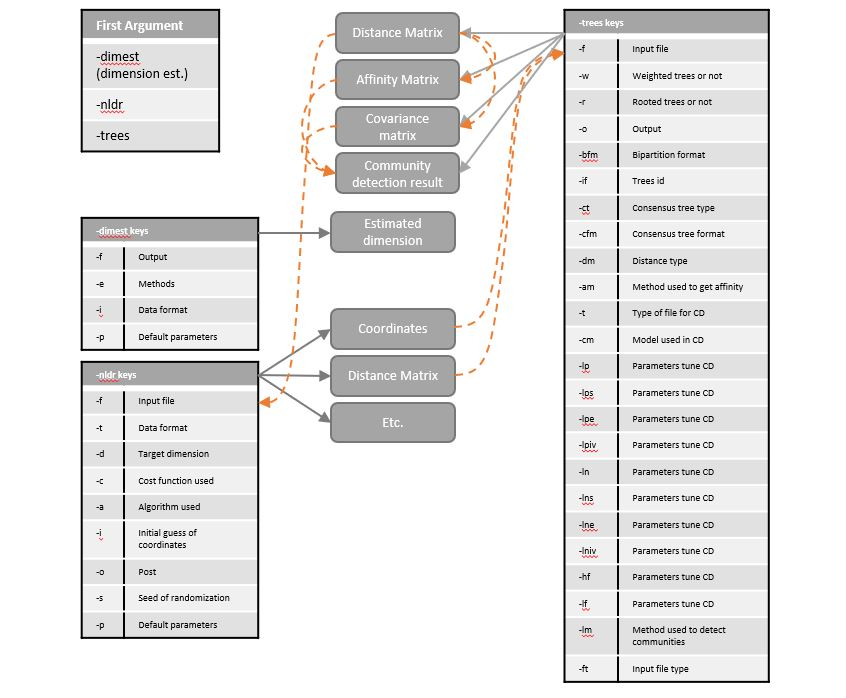
\includegraphics[width=\textwidth]{ArgumentList1.jpg}
		\caption{Argument List and routine structure of the current version.}
		\label{fig:argumentcurrent}
	\end{figure}
	
	TreeScaper binary takes a long command to execute a complicated task like performing community detection on a set of trees. The typical procedures TreeScaper is going to perform are
	\begin{enumerate}
		\item compute bipartition matrix of trees;
		\item compute trees distance matrix and affinity matrix or compute bipartition covariance matrix;
		\item perform community detection methods.
	\end{enumerate}
	

	These procedures are specified with one command like\\
	\texttt{./CLVTreeScaper -trees -f test.tre -ft trees -r 1 -w 1 -o Community -t Affinity -dm RF -cm CNM -lm auto}\\
	and produce bipartition matrix, affinity/covariance matrix and CD results, which is what the dashed line between output files from keyword \texttt{-trees}. Since these dependency happen internally in one command, we have no control over the intermediate results, i.e., modifications like manually setting threshold for affinity before CD is not possible.
	
	Such commands are inconvenient and also difficult to cooperate with the GUI system we are building on CloudForest. Therefore, keyword and command structure shown in Fig.\ref{fig:argumentnew} is proposed, while the old structure will remain in the TreeScaper binary until the new system become reliable. 
	

	\begin{figure}[!h]
		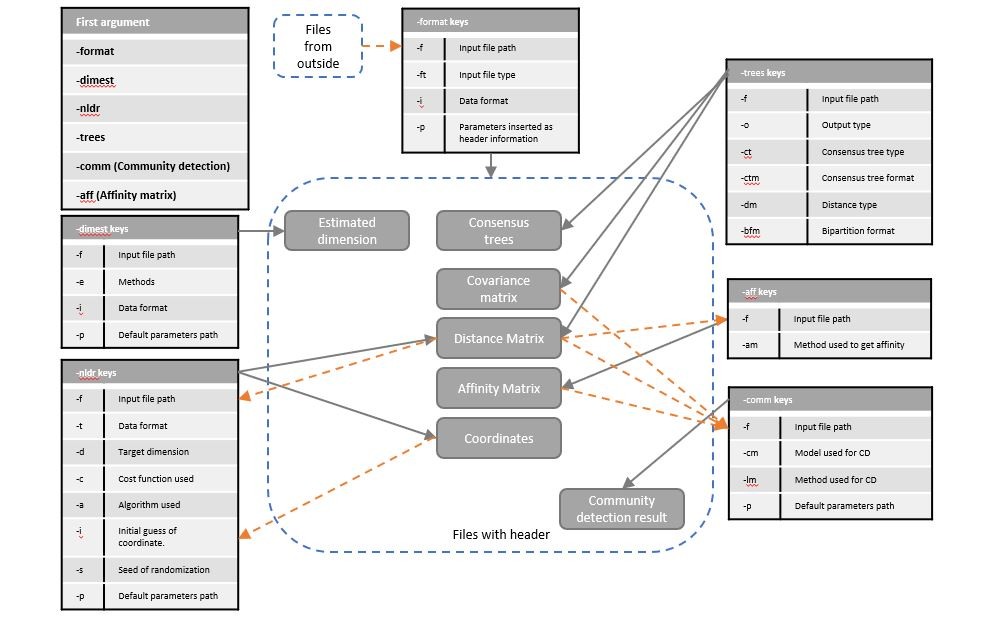
\includegraphics[width=\textwidth]{ArgumentList2.jpg}
		\caption{Argument List and routine structure of the new version.}
		\label{fig:argumentnew}
	\end{figure}

	New key arguments \texttt{-format}, \texttt{-comm} and \texttt{-aff} are added to TreeScaper. The new structure is centered at files with header information (in order to simplify file names and shorten argument list). \texttt{-format} takes care of converting files from other source with different format to files consistent with TreeScaper.
	
	\texttt{-aff} and \texttt{-comm} which stand for affinity and community detection are separated from \texttt{-tree}, which now only takes care of computing bipartition matrix, distance matrix and covariance matrix from tree file. Users are now able to perform any modification on output files from \texttt{-tree}, for example, send them to \texttt{-nldr}. Then \texttt{-comm} will take these (modified) files and other necessary information to perform CD methods.
	
	The specific argument list of these keys are given in following sections. Note that the current beta version of TreeScaper still accepts old commands, yet those keys are not suggested to use anymore and will also be \st{crossed} in the argument table.
	
	\clearpage
	\subsection{\texttt{-dimest} arguments}
	
	Currently, the key \texttt{-dimest} for dimensional estimation is a self-contained subroutine. It takes in a distance matrix $D$ or coordinates matrix $X$ of $n$ points $\{p_i\},i=1,\cdots,n$ and return the estimated rank of the matrix along with the analysis result. This could be used as an instruction on nonlinear dimension reduction task.
	
	\begin{table}[!h]
		\centering
		\begin{tabular}{cll}
			\hline
			Arguments & Description & options\\
			\hline
			\texttt{-f}& Source file &  \\
			\hline
			\texttt{-e}& Algorithm & \texttt{CORR\_DIM}, \texttt{NN\_DIM}, \texttt{EIG\_DIM}, \texttt{MLE\_DIM}\\
			\hline
			\texttt{-i}& Data type& \texttt{DIS}, \texttt{COR}\\
			\hline
			\texttt{-p}& Parameter file&\\
			\hline
		\end{tabular}
		\caption{Argument list of \texttt{-dimest}}
		\label{tab:dimestlist}
	\end{table}
	
	
	\subsection{\texttt{-nldr} arguments}
	
	The key \texttt{-nldr} takes in a distance matrix of $n$ points $p_i, i =1,\cdots, n$ on certain metric space and return coordinates of $\title{p}_i$, lies on Euclidean space $\mathbb{R}^k$ along with other useful information. In particular, the coordinates matrix $\tilde{C}$ of $\tilde{p}_i$ stores in \texttt{Coordinate.out} and the Euclidean distance matrix $\tilde{D}$ stores in \texttt{Distance.out}.
	
	\begin{table}[!h]
		\centering
		\begin{tabular}{cll}
			\hline
			Arguments & Description & options\\
			\hline
			\texttt{-f}& Source file &  \\
			\hline
			\texttt{-t}& Data type & \texttt{COR}, \texttt{DIS}\\
			\hline
			\texttt{-d}& Target dimension, $k$&\\
			\hline
			\texttt{-c}& Cost function& \texttt{CCA}, \texttt{SAMMON}, \texttt{CLASSIC\_MDS}\footnote{This method, classical scaling, only works when distance matrix are generated on classic Euclidean space $\mathbb{R}^n$.}\\
			&&\texttt{KRUSKAL1}, \texttt{NORMALIZED}\\
			\hline
			\texttt{-a}& Algorithm & \texttt{STOCHASTIC}, \texttt{METROPOLIS}, \texttt{GAUSS\_SEIDEL}\\
			&&\texttt{LINEAR\_ITERATION}, \texttt{MAJORIZATION}\\
			\hline
			\texttt{-i}& Initial guess & \texttt{RAND}, \texttt{CLASSIC\_MDS}\footnote{Use the result of classical scaling as initial guess.}\\
			\hline
			\texttt{\st{-o}}& \st{Output postfix}&\\
			\hline
			\texttt{-post} & Output postfix&\texttt{none}, \texttt{time}, \texttt{AnyString}\\
			\hline
			\texttt{-p}& Parameter file&\\
			\hline
		\end{tabular}
		\caption{Argument list of \texttt{-nldr}}
		\label{tab:nldrlist}
	\end{table}

	Note that \href{https://en.wikipedia.org/wiki/Multidimensional_scaling}{classical scaling}, the algorithm used to optimized the cost function \texttt{CLASSIC\_MDS} only works for Euclidean case, i.e., when $D$ is a Euclidean distance matrix on $\mathbb{R}^n$, which makes this method less desirable for our tree space. However, it can be used as a way to obtain a good enough initial guess for other methods. 
	
	Also notice that \texttt{-o} for output postfix label is dropped and you are recommend to use \texttt{-post} for creating standard filename like \texttt{Distance\_XXX.out}. The default \texttt{-post} is \texttt{time}, which will create file like \texttt{Distance\_m\_d\_hrs\_min.out}.
	
	\clearpage
	
	\subsection{\texttt{-trees} arguments}
	
	The key \texttt{-trees} is able to accomplish multiple tasks:
	\begin{enumerate}
		\item Distance: it takes in $n$ trees and return a distance matrix $D\in \mathbb{R}^{n \times n}$
		\item Affinity: it takes in $n$ trees or a distance matrix $D$ and return an affinity matrix $A$ computed from $D$ or certain distance matrix from the input trees set.
		\item Consensus tree: it takes in $n$ trees and return the consensus tree from input trees set.
		\item Covariance: it takes in $n$ trees and return the covariance matrix $\mathcal{R}\in \mathbb{R}^{m\times m}$ of $m$ bipartition appeared in the trees set.
		\item Community: it takes in affinity matrix or covariance matrix and perform the community detection method.
	\end{enumerate}

	Note that all tasks are coupled with each other if there is mathematical dependence. For example, when \texttt{-o Affinity} appears, \texttt{-trees} computes and outputs bipartition matrix, distance matrix and affinity matrix; when \texttt{-o Community -t Covariance} appears, \texttt{-trees} computes and outputs bipartition matrix, covariance matrix and community detection results.
	
	\begin{table}[!h]
		\centering
		\begin{tabular}{cll}
			\hline
			Arguments & Description & options\\
			\hline
			\texttt{-f}& Source file &  \\
			\hline
			\st{\texttt{-ft}}\footnote{This is dropped since CD is separated from \texttt{-trees} and we only read trees now.}& \st{Data type} & \st{\texttt{Trees}, \texttt{Cova}}\\
			\hline
			\texttt{-w}& Weighted tree flag&\\
			\hline
			\texttt{-r}& Rooted tree flag& \\
			\hline
			\texttt{-o}& Output type & \texttt{Dist}, \texttt{Cova}, \texttt{Consensus}\\
			&&\st{\texttt{Affinity}, \texttt{Community}}\\
			\hline
			\texttt{-bfm}& Bipartition output format & \texttt{list}, \texttt{matrix}\\
			\hline
			\texttt{-if}& Tree id file&\\
			\hline
			\texttt{-ct}& Consensus Tree type& \texttt{Majority}, \texttt{Strict}\\
			\hline
			\texttt{-ctm}& Consensus Tree format& \texttt{Nexus}, \texttt{Newick}\\
			\hline
			\texttt{-dm}& Distance type& \texttt{RF}, \texttt{URF}, \texttt{Mat}, \texttt{SPR}\\
			\hline
			\st{\texttt{-am}}& \st{Affinity type}& \st{\texttt{Rec}, \texttt{Exp}}\\
			\hline
			\st{\texttt{-cm}}& \st{Community detection method}& \st{\texttt{CNM}, \texttt{CPN}, \texttt{ERNM}, \texttt{NNM}}\\
			\hline
			\st{\texttt{-lm}}& \st{Community detection} & \st{\texttt{auto}, \texttt{manu}}\\
			& \st{parameter setting}&\\
			\hline
			\st{\texttt{-t}}& \st{Type of label used in} & \st{\texttt{Affinity}, \texttt{Covariance}}\\
			& \st{community detection}&\\
			\hline
			\texttt{-post} & Output postfix&\texttt{none}, \texttt{time}, \texttt{AnyString}\\
			\hline
		\end{tabular}
		\caption{Argument list of \texttt{-trees}}
		\label{tab:treeslist}
	\end{table}
	
	\clearpage
	
	\subsection{\texttt{-aff} arguments}
	
	The key \texttt{-aff} takes in any distance matrix $D$ and return affinity matrix $A$ computed from $D$.
	
	
	\begin{table}[!h]
		\centering
		\begin{tabular}{cll}
			\hline
			Arguments & Description & options\\
			\hline
			\texttt{-f}& Source file &  \\
			\hline
			\texttt{-am}& Affinity type & \texttt{Rec}, \texttt{Exp}\\
			\hline
			\texttt{-post} & Output postfix&\texttt{none}, \texttt{time}, \texttt{AnyString}\\
			\hline
		\end{tabular}
		\caption{Argument list of \texttt{-aff}}
		\label{tab:aff}
	\end{table}
	
	\subsection{\texttt{-comm} arguments}
	
	The key \texttt{-comm} takes in any adjacency matrix $A$ from a graph and performs community detection algorithm on it. This matrix is usually assumed to be a covariance matrix of bipartitions from a set of trees or an affinity matrix from distance matrix of a set of trees. The former constructs a graph with bipartition as nodes and the latter constructs one with trees as nodes. However, generally $A$ can be an adjacency matrix of any kind of weighted non-directed graph. Therefore, the key accepts argument to set the node type as well.
	
		\begin{table}[!h]
		\centering
		\begin{tabular}{cll}
			\hline
			Arguments & Description & options\\
			\hline
			\texttt{-f}& Source file &  \\
			\hline
			\texttt{-cm}& Community Detection method & \texttt{CNN}, \texttt{CPM}, \texttt{ERNM}, \texttt{NNM}\\
			\hline
			\texttt{-lm}& Parameter tuning\footnote{Set $\lambda^+_{\min}$ and $\lambda^+_{\max}$ manually or automatically.}& \texttt{auto}, \texttt{manu}\\
			\hline
			\texttt{-node}& Node type& \\
			\hline
			\texttt{-post}& Output postfix & \texttt{none}, \texttt{time}, \texttt{AnyString}\\
			\hline
			\texttt{-hf}\footnote{Upper bound for removing highly connected nodes}& Tunning parameter&\\
			\hline
			\texttt{-lf}\footnote{lower bound for removing merely connected nodes}& Tunning parameter&\\
			\hline
			\texttt{-lp}& Manual Tunning parameter&\\
			\hline
			\texttt{-ln}& Manual Tunning parameter&\\
			\hline
			\texttt{-lps}& Manual Tunning parameter& \\
			\hline
			\texttt{-lpe}& Manual Tunning parameter&\\
			\hline
			\texttt{-lpiv}& Manual Tunning parameter&\\
			\hline
			\texttt{-lns}& Manual Tunning parameter&\\
			\hline
			\texttt{-lne}& Manual Tunning parameter&\\
			\hline
			\texttt{-lniv}& Manual Tunning parameter&\\
			\hline
		\end{tabular}
		\caption{Argument list of \texttt{-comm}}
		\label{tab:commlist}
	\end{table}

	Note that the arguments for manually tuning CD will later be combine into a \texttt{parameter\_comm.csv}. 
	
	\subsection{\texttt{-format} arguments}
	
	\subsection{Command example}
	
	In this part, we give some example of calling TreeScaper for different tasks in order to help you understand the new command structure. All commands mentioned here can be found in the file \texttt{command\_example.txt}.
	
	Suppose there is a tree file \texttt{boottrees.nhx} on the root directory as well as on a sub directory. 
	
	\textbf{Perform a community detection on trees based on particular distance.}
	
	The old command in one line is
	
	\texttt{./CLVTreeScaper -trees -f boottrees.nhx -ft Trees -w 1 -r 0 -o Community -dm RF -t Affinity -am Rec -cm Auto -hf 0.9 -lf 0.1}
	
	Note that the old command requires the tree file be in the same directory of the binary file. This command will sequentially generates bipartition file, distance file, affinity file and the final community detection result.
	
	For the beta version, you are suggested to use the following set of commands to call CLVTreeScaper multiple times. Notice that the new command allows input and output in directory other than the current one.
	
	\begin{enumerate}
		\item \texttt{./CLVTreeScaper -trees -f sub\_dir/boottrees.nhx -w 1 -r 0 -o Dist -dm RF -post test}
		
		It generates bipartition output and a distance matrix in \texttt{sub\_dir/Distance\_test}.
		
		\item' If you want to further process the distance matrix with \texttt{-nldr}, call
		
		\texttt{./CLVTreeScaper -nldr -f sub\_dir/Distance\_test.out -t DIS -d 20 -c CCA -a STOCHASTIC -i RAND -post NLDR\_test}
		
		It generates a coordinates matrix \texttt{sub\_dir/Coordinate\_NLDR\_test.out} and a distance matrix \texttt{sub\_dir/Distance\_NLDR\_test.out}. This step is not necessary.
		
		\item \texttt{./CLVTreeScaper -aff -f sub\_dir/Distance\_NLDR\_test.out -am Rec -post NLDR\_test}
		
		It generates an affinity matrix \texttt{sub\_dir/Affinity\_NLDR\_test.out}.
		
		\item \texttt{./CLVTreeScaper -comm -f example/Affinity\_NLDR\_test.out -lm auto -hf 0.9 -lf 0.1}
		
		It performs the final community detection method on the graph based on affinity matrix. 
	\end{enumerate}

	Note that you may perform NLDR method multiple times if necessary. Also note that you can further modify every files manually or with other software (as long as the format is maintained) before going to the next step. This is not recommended unless you are sure about the modification serves for your purpose.

	\textbf{Perform a community detection of bipartition based on covariance matrix.}
	
	The old one-line command for this task is
	
	\texttt{./CLVTreeScaper -trees -f boottrees.nhx -ft Trees -w 1 -r 0 -o Community -t Covariance -am Rec -cm Auto -hf 0.9 -lf 0.1}
	
	This command will sequentially generates bipartition file, covariance file and the final community detection result.
	
	For the beta version, you are suggested to use the following set of commands to call CLVTreeScaper multiple times.

	\begin{enumerate}
		\item \texttt{./CLVTreeScaper -trees -f sub\_dir/boottrees.nhx -w 1 -r 0 -o Cova -post test}
		
		It generates bipartition output and a distance matrix in \texttt{sub\_dir/Covariance\_test}.
		
		\item \texttt{./CLVTreeScaper -comm -f example/Covariance\_test.out -lm auto -hf 0.9 -lf 0.1}
		
		It performs the final community detection method on the graph based on covariance matrix. 
	\end{enumerate}

	
	\subsection{Header information}
	
	The beta version of TreeScaper are now centered at the output files of each subroutine. Different subroutines communicate through the formatted header information in the file they read and the file they output. (\textbf{WARNING}: Header in tree file and \texttt{-dimest} is NOT supported.)
	
	Here is a typical header information from a distance matrix created by \texttt{-nldr}:
	\\
	\texttt{<}
	\\
	\\
	\texttt{created:8\_3\_0\_33}
	\\
	\texttt{output\_type:Distance matrix}
	\\
	\texttt{distance\_type:Robinson-Foulds}
	\\
	\texttt{node\_type:Tree}
	\\
	\texttt{node\_feature:weighted, unrooted, NLDR(20)}
	\\
	\texttt{source:example/ATP8.tre}
	\\
	\\
	\texttt{>}
	
	It is multiple lines of string inside a angle bracket. The information is stored as \texttt{map<String, String>} inside TreeScaper, such that each line gives a pair of \texttt{key-value} separated by the colon '\texttt{:}'. These header information are formatted in human-readable fashion. The \texttt{key} usually have no space and the \texttt{value} may have more than one item, separated by '\texttt{, }'.
	
	When a subroutine read a file with header, it will load in all header information, update or drop certain lines and then make use of some of them. Finally, the routine will add more information to the header and print it on the output file. Therefore, you may insert information you need in the format of \texttt{KEY:VALUE} and it will present in later files.
	
	\section{Basic data structures}
	
	Most of the basic data structures are constructed by Wen Huang. They includes basic array, matrix, string, mapping and file stream. They are, basically the c++ built-in structure warped up with convenient functions and operators. For example, the matrix class integrates singular value decomposition from CLAPACK. These data structures' header file and implementation files are prefixed with "w".
	
	There are other more complicated data structures for specific algorithm and mathematical objects such as trees and community. They will be addressed in the next section. 
	
	\subsection{Array}
	
	Members of array of type \ttype{T} are consisted of a pointer of \ttype{T}* \texttt{vec} and a static integer \texttt{length} that indicates the length. The member functions and operators are given below.
	
	\begin{enumerate}
		\item \texttt{friend std::istream \&operator>>}
		
		This operator does nothing and will not assign value to the array from the \texttt{istream}. According to particular needs of reading data, this may later be implemented with actual reading functionality.
		
		\item \texttt{friend std::ostream \&operator<<}
		
		This operator will output the length and its components separated by ":" and ",".
		
		Example: an array of \ttype{char[]} from "a" to "e" is outputted in the format of
		
		\texttt{\{ 5 : a, b, c, d, e\}}
		
		\item \texttt{const Array\& Array::operator=(const Array \&right)}
		
		The assignment operator will free the pointer \texttt{vec} on the left and allocate a new \texttt{vec}. Then it assigns values from right hand side to left hand side component-wise. 
		
		The operator returns a pointer of the array on the left.
		
				
		\item \texttt{const Array\& Array::operator+=(const Array \&right)}
		
		This operator creates a new array with the right hand side attached to left hand side. It allocates \texttt{Array} of the correct length and then assigns values accordingly. Then call the assignment operator \texttt{=} to overwrite the current array.
		
		Warning: calling \texttt{=} costs repeated and unnecessary copy-pasting.
		
		\item \texttt{const Array\& Array::operator-=(const Array \&right)}
		
		This operator creates a new array from the left hand side, with every component presented in the \texttt{right} removed and calls assignment operator to overwrite the current \texttt{Array}.
		
		Warning: calling \texttt{=} costs repeated and unnecessary copy-pasting. 
		
		Warning: the new array is built incrementally and calls \texttt{resize} everytime, will brings the complexity to $O(length^2\times right.length)$ other than $O(length\times right.length)$.
		
		\item \texttt{bool Array::operator==}
		
		Compares two array component-wise after comparing the length.
		
		\item \texttt{bool Array::operator<}
		
		The logic of the compare operator is to set the array with component-wise greater component to be the greater one. If the lengths are different, only compare the first $k$ components where $k$ is the smaller length. If the first $k$ components happens to be the same (component-wise), the longer \texttt{Array} is greater than the shorter one. 
		
		\item \texttt{Array Array::operator(const int index, const int end)}
		
		This operator extract sub-array from the current array. It takes two indices as parameters and return a new array that has the values from \texttt{index} to \texttt{end}.
		
		Warning: this implementation is different than the implementation of \texttt{String::operator()}, which also takes two integers as parameters but the first one is the starting index and the second one is the length of the sub-string, instead of the ending index.
		
	\end{enumerate}
	
	\subsection{Matrix}
	
	Members of a matrix of type \ttype{T} are consisted of a pointer of pointers \ttype{T}** implemented in\href{https://en.wikipedia.org/wiki/Row-_and_column-major_order}{row-major} and two static integers \texttt{row} and \texttt{col} which indicate the dimensions of the matrix. This class also calls classic linear algebra algorithms from \href{https://www.netlib.org/clapack/}{CLAPACK}. 
	
	Overloaded operators are given below.
	
	\begin{enumerate}
		\item \texttt{friend istream \&operator>>}.
		
		Warning: This operator does nothing, i.e., it does not assign values from the input stream.
		\item \texttt{friend ostream \&operator<<}.
		
		This operator output the matrix in the format of
		
		\texttt{\{ ( 3 , 2 )}
		
		\texttt{a, b, c}
		
		\texttt{d, e, f}
		
		\texttt{\}}
		\item \texttt{friend Matrix operator+(Matrix<\ttype{T}> left, Matrix<\ttype{T}> right)}.
		
		This operator resize the left and right matrices to the lager dimension by calling member function \tref{resize}{MatrixResize} and then create a new matrix and assign values from entry-wise addition.
		
		Warning: the resize of left and right is silent here, which will permanently change the matrix being summed.
		
		\item \texttt{friend Matrix operator+(Matrix<\ttype{T}> left, \ttype{S} right)}.
		
		This operator accepting a number \texttt{right} of type \ttype{S} on the right will add \texttt{right} entry-wise to each element in Matrix \texttt{left}, i.e., shift the matrix by \texttt{right}.
		
		\item \texttt{friend Matrix operator+(S left, Matrix<T> right)}
		
		Shift the matrix by \texttt{left} entry-wise.
		
		\item \texttt{friend Matrix operator-}
		
		See \texttt{friend Matrix operator+}.
		
		\item \texttt{Matrix operator*(const Matrix<\ttype{T}> \&left, const Matrix<\ttype{T}> \&right)}
		
		Implement \href{https://en.wikipedia.org/wiki/Matrix_multiplication}{matrix multiplication}.
		
		\item \texttt{friend Matrix operator*(\ttype{S} value, Matrix<\ttype{T}> mat)} or \texttt{(Matrix<\ttype{T}> mat, \ttype{S} value)}.
		
		This operator return a new matrix entry-wise scaled by \texttt{value}. Note that this operator does not change the original matrix.
		
		Warning: the matrix getting rescaled should be passed by reference in order to avoid construction/destruction computation.
		
		\item \texttt{friend Matrix operator/(Matrix<\ttype{T}> mat, \ttype{S} value)}
		
		This operator return a new matrix entry-wise divided by \texttt{value}. Note that this operator does not change the original matrix. Also note that this is not the syntax used in some advanced language where $A/B$ means $B^{-1}A$.
		
		Warning: the matrix getting rescaled should be passed by reference in order to avoid construction/destruction computation.
		
		\item \texttt{T \&operator()(const int r, const int c = 0)}
		
		This operator returns the entry at $r$-row and $c$-column.
		
	\end{enumerate}

	Important member functions are given below.
	
	\begin{enumerate}
		\item \texttt{Matrix<\ttype{double}> compute\_scalar\_product\_matrix()}
		
		This function return a \ttype{double} type matrix $S\in \mathbb{R}^{n\times n}$ from the current matrix $D^{(2)}\in \mathbb{R}^{n\times n}$. $S$ is the centering-scaled $D^{(2)}$, which is assumed to be a squared distance matrix of $n$ points $\{p_i\}_{i=1,\cdots, n}$, $D^{(2)}_{ij}=D^{(2)}_{ji}=d^2(p_i,p_j)$. 
		
		Note that the classical multidimensional scaling method, \href{https://en.wikipedia.org/wiki/Multidimensional_scaling}{MDS} assumes these $n$ points lie on some Euclidean space $\mathbb{R}^k$ equipped with classic 2-norm distance. And $S$ is a squared distance matrix of transformed $n$ points such that the arithmetic mean of new points is $0^k\in \mathbb{R}^k$. Also note that the arithmetic mean in Euclidean space is also the Karcher mean defined by
		\[
			\arg\min\limits_{m\in \mathbb{R}^k}\sum_{i=1}^n d^2(p_i,m).
		\]
		
		The formula of computing $S$ is given by
		\[
			S=-\frac{1}{2}JD^{(2)}J
		\]
		where $J=I-\frac{1}{n}\mathbf{1}\mathbf{1}^T$ and $\mathbf{1}\mathbf{1}^T$ is all-1 matrix. Also note that the transformation $D^{(2)}\to S$ preserves the solution of MDS, i.e.,
		\[
			\arg\min\limits_{B\in \mathbb{R}^{n\times k}} \left\Vert BB^T - D^{(2)}\right\Vert^2_F = \arg\min\limits_{B\in \mathbb{R}^{n\times k}} \left\Vert -\frac{1}{2}JBB^TJ + \frac{1}{2}JD^{(2)}J\right\Vert^2_F
		\]
		where $B$ is the Euclidean coordinate matrix of $n$ points in $\mathbb{R}^k$ which generates (approximately) the squared distance matrix $D^{(2)}$.
		
		Error: The invariance of transformation seems to be only true for Euclidean space. For more abstract $D^{(2)}$ generated from more general metric on Riemannian manifold, the scaling $-\frac{1}{2}JD^{(2)}J$ does not preserves positive definiteness of the squared distance matrix, which further causes negative eigenvalues in the following PCA, the eigendecomposition, process.
		
		Warning: The squared distance matrix $D^{(2)}$ used in here is inconsistent with the distance matrix $D$ computed in 
		%\mmemref{compute\_Distance\_Matrix}{computeDistanceMatrix},
		\texttt{compute\_Distance\_Matrix} in difference of entry-wise squared or not. 
		
		\item \texttt{Matrix<double> compute\_Distance\_Matrix()}
		
		This function return a \ttype{double} type matrix $D\in \mathbb{R}^{n\times n}$ computed from the current matrix $M\in \mathbb{R}^{n\times k}$. $M$ is consider as coordinate matrix of $n$ points in $k$-dimensional Euclidean space, $i$-th row represents the $k$-tuple Euclidean coordinates of a point $p_i$. And $D$ is the distance matrix where $D_{ij}=D_{ji}=d(p_i,p_j)=\Vert p_i - p_2j\Vert_2$ is the 2-norm distance between points $p_i,p_j$.
		
		Warning: the resulting distance matrix $D$ is dense, the symmetric structure is not exploited here. 
	\end{enumerate}

	\section{Algorithms}
	
	\subsection{Nonlinear dimensional reduction(NLDR)}
	
	This part collects algorithms and their important subroutines implemented in TreeScaper. The main goal in these algorithms is that given a squared distance matrix $D^{(2)}$ or distance matrix $D$ of $n$ points $\{p_i\}_{i=1,\cdots, n}$ on some metric space, find $n$ points $\{p_i'\}_{i=1,\cdots,n}\subset \mathbb{R}^k$, such that the distance matrix $D'$ for $\mathbf{p}'$ approximates $D$ the best, under the cost functions defined in different algorithm. Note that these $n$ new points $\mathbf{p}'$ can be represents by the coordinate matrix $B\in \mathbb{R}^{n\times k}$ which is often used as the output of these NLDR algorithms.
	
	\subsubsection{Classical Multidimensional scaling(MDS)}.
	
	Classical Multidimensional scaling assumes $D^{(2)}$ is generated from Euclidean space with typical vector 2-norm as distance. The implemented algorithm \texttt{NLDR::CLASSIC\_MDS} contains 4 parts:
	\begin{enumerate}
		\item Compute centered matrix $S$ from the given tree distance matrix $D$ by calling 
		
		\rref{Matrix}::\mtref{compute\_Scalar\_Matrix}{MatrixComputeScalarMatrix}.
		\item Perform \href{https://en.wikipedia.org/wiki/Singular_value_decomposition}{singular value decompositions(SVD)} to $S$ by calling \rref{Matrix}::\mtref{SVD\_LIB}{MatrixSVDLIB} to obtain
		\[
			S = U\Sigma V^T.
		\]
		
		Note that since $S$ is symmetric, there exist eigen-decomposition $S=Q\Lambda Q^T$, i.e., there exists a signature matrix $E$, which has only $1$ or $-1$ in diagonal and $0$ elsewhere, such that $U\Sigma V^T = Q\Lambda EEQ^T=Q(\Lambda E)(QE)^T$ and $U = Q$, $\Sigma = \Lambda E$ and $V = QE$. This implies eigen-decomposition from CLAPACK is more efficient.
		
		Also note that if $D^{(2)}$ uses vector 2-norm in Euclidean space, $S$ is positive definite and SVD coincides with eigen-decomposition.
		
		Warning: when there exist files named consistently that indicates SVD has been done and $U,V,\Sigma$ has been stored, the routine will not do it again but simply read them from files. This is silent and could cause problem if those files are not actually inconsistent.
		\item In case of performing MDS for $D^{(2)}$ from other metric space, which cause the presence of negative eigenvalues, it selects the $k$ eigenvectors $Q_{i_j}$, $j=1,\cdots k,$ where $\lambda_{i_j}$ are the $k$ most largest positive eigenvalues.
		
		Error: memory leakage happens in this process whenever a negative eigenvalues encountered in the $k$ most largest in magnitude eigenvalues. This problem is temporarily fixed but the theoretical explanation and necessity of this process is still needed. the classical MDS may not be suitable at all for Tree subjects.
		
		\item Produce the coordinates matrix $B$ for $n$ points $\mathbf{p}'\subset \mathbb{R}^{k}$ by
		\[
			B=\begin{bmatrix}
				\sqrt{\lambda_{i_1}}Q_{i_1} & \cdots & \sqrt{\lambda_{i_k}}Q_{i_k}
			\end{bmatrix}\in \mathbb{R}^{n\times k}.
		\]
		
		\item Compute the stress that estimate how good $BB^T$ approximate $D^{(2)}$ by calling \rref{NLDR}::\mtref{CLASSIC\_MDS\_stress\_function}{NLDRCLASSICMDSstressfunction}.
		
		Note that classical MDS do not need to compute the stress since $B$ already minimized the stress function. However, since Tree space is not a Euclidean space with appropriate distance, the output $B$ does not minimize the stress function.
	\end{enumerate}
	
	
	
	For more information of MDS, see \href{https://en.wikipedia.org/wiki/Multidimensional_scaling}{here}.
	
	\section*{Implementations of some routines}
	
	
	\section*{Data structure}
	
	
	\begin{enumerate}
		\item \mrref{Matrix}
			
			\begin{tabular}{>{\bfseries}lp{0.2\textwidth}p{0.6\textwidth}}
				Description & \multicolumn{2}{p{0.8\textwidth}}{Row-major 2-dimensional array.} \\
				Member & \mtref{row}{MatrixRow} & Number of rows.\\
				&\mtref{col}{MatrixCol} & Number of columns.\\
				&**\mmemref{matrix}{MatrixMatrix} & Pointers to each row.\\
				Member function& \tref{resize}{MatrixResize} & Change the dimensions. \\
			\end{tabular}
		
		\item \mrref{Ptree}
		
			\begin{tabular}{>{\bfseries}lp{0.2\textwidth}p{0.6\textwidth}}
				Description & \multicolumn{2}{p{0.8\textwidth}}{Index base array-type unweighted tree with adjacency matrix.} \\
				Member & \mtref{leaf\_number}{leafnumber} &\\
				&*\mmemref{parent}{Ptree} & Array of indices of the parent.\\
				&*\mmemref{lchild}{Ptree} & Array of indices of the right child.\\
				&*\mmemref{rchild}{Ptree} & Array of indices of the left child.\\
				&**\mmemref{edge}{Ptree}  & Adjacency matrix.\\
				Member function& none &  \\
			\end{tabular}
		
		\item \mrref{NEWICKNODE}
		
			\begin{tabular}{>{\bfseries}lp{0.2\textwidth}p{0.4\textwidth}}
				Description & \multicolumn{2}{p{0.6\textwidth}}{Linked node pointed to its children and parent.} \\
				Member & \mmemref{Nchildren}{NEWICKNODE}  & Number of children.\\
				& \mmemref{label}{NEWICKNODE} &\\
				& \mmemref{weight}{NEWICKNODE} &\\
				& *\mmemref{child}{NEWICKNODE} & List of children.\\
				& \mmemref{hv1}{NEWICKNODE} & Hash value for unknown use.\\
				& \mmemref{hv2}{NEWICKNODE} & Hash value that identifies the bipartition.\\
				& \mmemref{bitstr}{NEWICKNODE} & Bit string that represents the leaves contained in the (sub-)tree.\\
				& \mmemref{parent}{NEWICKNODE} & \\
				Member function& none  &  \\
			\end{tabular}

		
		\item \mrref{NEWICKTREE}
		
			\begin{tabular}{>{\bfseries}lp{0.2\textwidth}p{0.4\textwidth}}
				Description & \multicolumn{2}{p{0.6\textwidth}}{A \rref{NEWICKNODE} that represents the root.} \\
				Member & \mmemref{root}{NEWICKTREE}  & A \rref{NEWICKNODE}.\\
				Member function& none  &  \\
			\end{tabular}

		
		\item \mrref{TreeOPE}
		
			\begin{tabular}{>{\bfseries}lp{0.2\textwidth}p{0.4\textwidth}}
				Description & \multicolumn{2}{p{0.6\textwidth}}{Operation associated to one \rref{NEWICKTREE}. Note that most of the method are implemented in recursive preorder.} \\
				Member &   & \\
				&   &\\
				Member function& \rref{loadnewicktree} &  Read \rref{NEWICKTREE}.\\
				& \rref{loadnewicktree2} & Read \rref{NEWICKTREE}.\\
				& \rref{floadnewicktree} & Read \rref{NEWICKTREE}.\\
				& \rref{loadnode} & Read \rref{NEWICKTREE}.\\
				& \rref{loadleaf} & Read \rref{NEWICKTREE}.\\
				& \rref{parsetree} & Read \rref{NEWICKTREE}.\\
				& \rref{parsenode} & Read \rref{NEWICKTREE}.\\
				& \rref{parseleaf} & Read \rref{NEWICKTREE}.\\		
				& \rref{addchild} & Link child to the parent.\\
				& \tref{dfs\_compute\_hash}{dfscomputehash}  &  Assigned hash values to all (sub-)tree which identifies the structure and therefore the bipartition.\\
				& \rref{bipart} & Store hash values in one big array for computing RF distance.\\
				& \rref{findleaf} & Find a leaf by the \memref{label}{NEWICKNODE}.\\
				& \rref{normalizedTree} & Lift a unrooted tree to a rooted tree.\\
				& \rref{newick2lcbb} & Convert \rref{NEWICKTREE} to \rref{Ptree} for computing matching distance.\\
				& \rref{newick2ptree} & Implementation of \rref{newick2lcbb}.\\
				& \rref{sumofdegree} & \\
				& \rref{bipartcount} & Count the occurrence of particular bipartition.\\
				& \rref{Addbipart} & Insert nodes to the current tree so that there exist a (sub-)tree that contains only a given set of leaves.
				
			\end{tabular}

		\item \mrref{Trees}
		
			\begin{tabular}{>{\bfseries}lp{0.3\textwidth}p{0.3\textwidth}}
				Description & \multicolumn{2}{p{0.6\textwidth}}{Multiple \rref{NEWICKTREE}s with member function that computes different distances.} \\
				Member &   & \\
				Member function & \rref{initialTrees} & Read trees from file. \\
				& \rref{ReadTrees} & Read trees from file. \\
				& \tref{compute\_numofbipart}{computenumofbipart} & \\
				& \tref{Compute\_Hash}{ComputeHash} & Generate hash table for computing hash values in a tree.\\
				& \tref{Compute\_Bipart\_Matrix}{ComputeBipartMatrix} & Generate a sparse matrix that stores the weight of bipartition, its frequency of occurrence.\\
				& \tref{Compute\_Bipart\_Covariance}{ComputeBipartCovariance} & Generate the covariance matrix according to the formula.\\
				& \tref{Compute\_RF\_dist\_by\_hash}{ComputeRFdistbyhash} & Generate the RF-distance matrix according to the formula.\\
				& \rref{pttree} & Construct the adjacency matrix of a \rref{Ptree}.\\
				& \tref{compute\_matrix}{computematrix} & Generate matrix for computing matching distance by accumulating common edges from two \rref{Ptree}s.\\
				& \tref{Compute\_Matching\_dist}{ComputeMatchingdist} & Compute the matching distance between two trees by the XOR table created from all possible bipartitions.\\ 
				& \tref{Compute\_Affinity\_dist}{ComputeAffinitydist} & Compute the affinity distance from the given distance matrix.\\
			\end{tabular}
	
		
	\end{enumerate}


	
	\subsection*{\texttt{\texttt{TreeOPE}} related routines.}
	\begin{enumerate}
		\item \rref{TreeOPE}::\mrref{loadnewicktree}.
		
		\begin{tabular}{>{\bfseries}lp{0.2\textwidth}p{0.4\textwidth}}
			\hline
			Argument & \multicolumn{2}{p{0.6\textwidth}}{\texttt{(char *fname, int *error)}} \\
			\hline
			Description & \multicolumn{2}{p{0.6\textwidth}}{Read tree from formatted string that stores bipartition. The implementation is given in \rref{floadnewicktree}. Same level of the node is paired by "()" and separated by ",".
			} \\
			\hline
			Complexity&   &  \\
			Memory space&   &  \\
			\hline
			Associated routine& \rref{floadnewicktree} & Implementation by recursive processing the string in preorder.\\
			\hline
			Comments & \multicolumn{2}{p{0.6\textwidth}}{This routine is better implemented by stack structure. It can only process unweighted tree. Also this routine takes the file name as input while the duplication version \rref{loadnewicktree2} takes FILE type, customized fstream type. This routine seems to be insecure and redundant.} \\
			\hline
			Error code & -1 & Out of memory.\\
			& -2 & Parse error, the parentheses in string does not match.\\
			\hline
		\end{tabular}
	
		\item \rref{TreeOPE}::\mrref{loadnewicktree2}.
		
		\begin{tabular}{>{\bfseries}lp{0.3\textwidth}p{0.3\textwidth}}
			\hline
			Argument & \multicolumn{2}{p{0.6\textwidth}}{\texttt{(FILE *fp, int *error)}} \\
			\hline
			Description & \multicolumn{2}{p{0.6\textwidth}}{Duplication version of \rref{loadnewicktree} but with customized fstream. Actual implementation is not given in here, but in \rref{floadnewicktree}} \\
			\hline
			Complexity&   &  \\
			Memory space&   &  \\
			\hline
			Associated routines & \rref{floadnewicktree} & Implementation by recursive processing the string in preorder.\\
			\hline
			Comments & \multicolumn{2}{p{0.6\textwidth}}{This routine also seems to be redundant since the main thread of TreeScaper never called it. There is another input routine \rref{parsetree}, which can handle both weighted and unweighted tree, is used in TreeScaper.} \\
			\hline
			Error code & -1 & Out of memory.\\
			& -2 & Parse error, the parentheses in string does not match.\\
			\hline
		\end{tabular}
		
		
		\item \rref{TreeOPE}::\mrref{floadnewicktree}.
		
		\begin{tabular}{>{\bfseries}lp{0.2\textwidth}p{0.4\textwidth}}
			\hline
			Argument & \multicolumn{2}{p{0.6\textwidth}}{\texttt{(FILE *fp, int *error)}} \\
			\hline
			Description & \multicolumn{2}{p{0.6\textwidth}}{A pair of nodes are created by \rref{loadnode} when "(" is encountered.} \\
			\hline
			Complexity&   &  \\
			Memory space&   &  \\
			\hline
			Associated routine& \rref{loadnode} & \\
			\hline
			Comments & \multicolumn{2}{p{0.6\textwidth}}{This routine also seems to be redundant since the main thread of TreeScaper never called it. There is another input routine \rref{parsetree}, which can handle both weighted and unweighted tree, is used in TreeScaper.} \\
			\hline
			Error code & -1 & Out of memory.\\
			& -2 & Parse error, the parentheses in string does not match.\\
			\hline
		\end{tabular}
	
		\item \rref{TreeOPE}::\mrref{loadnode}.
		
		\begin{tabular}{>{\bfseries}lp{0.25\textwidth}p{0.35\textwidth}}
			\hline
			Argument & \multicolumn{2}{p{0.6\textwidth}}{\texttt{(FILE *fp, int *error)}} \\
			\hline
			Description & \multicolumn{2}{p{0.6\textwidth}}{Create internal nodes. When this function is called, a "(" has been read, if \texttt{fp} continue to read "(", next pair of nodes should be generated, i.e., \rref{loadnode} is called again, otherwise a leaf is encountered and \rref{loadleaf} will be called. When ")" is encountered, it is at the end of the current pair of nodes and should exit the routine to returned to previous level of node.} \\
			\hline
			Complexity&   &  \\
			Memory space&   &  \\
			\hline
			Associated routine& \mrref{loadleaf} & Add a leaf and return to previous level.\\
			& \mrref{addchild} & Add the new pair of nodes to their parent.\\
			& \mrref{readlabelandweight} & Read additional information from string.\\
			\hline
			Comments & \multicolumn{2}{p{0.6\textwidth}}{This is better implemented by stack structure. Also note that this method read leaves in preorder traversal.} \\
			\hline
			Error code & -1 & Out of memory.\\
			& -2 & Parse error, the parentheses in string does not match.\\
			\hline
		\end{tabular}
		
		\item \rref{TreeOPE}::\mrref{parsetree}.
		
		\begin{tabular}{>{\bfseries}lp{0.2\textwidth}p{0.4\textwidth}}
			\hline
			Argument & \multicolumn{2}{p{0.6\textwidth}}{\texttt{(char *str, int *error, NEWICKTREE *testtree)}} \\
			\hline
			Description & \multicolumn{2}{p{0.6\textwidth}}{Duplicate version of \rref{floadnewicktree}.} \\
			\hline
			Complexity&   &  \\
			Memory space&   &  \\
			\hline
			Associated routine& \rref{parsenode} & \\
			\hline
			Comments & \multicolumn{2}{p{0.6\textwidth}}{This is the routine used in TreeScaper.} \\
			\hline
			Error code & -1 & Out of memory.\\
			& -2 & Parse error, the parentheses in string does not match.\\
			\hline
		\end{tabular}
	
		\item \rref{TreeOPE}::\mrref{parsenode}.
		
		\begin{tabular}{>{\bfseries}lp{0.25\textwidth}p{0.35\textwidth}}
			\hline
			Argument & \multicolumn{2}{p{0.6\textwidth}}{\texttt{(FILE *fp, int *error)}} \\
			\hline
			Description & \multicolumn{2}{p{0.6\textwidth}}{Duplicated version \rref{loadnode}.} \\
			\hline
			Complexity&   &  \\
			Memory space&   &  \\
			\hline
			Associated routine& \mrref{parseleaf} & Add a leaf and return to previous level.\\
			& \mrref{addchild} & Add the new pair of nodes to their parent.\\
			& \mrref{parselabelandweight} & Read additional information from string.\\
			\hline
			Error code & -1 & Out of memory.\\
			& -2 & Parse error, the parentheses in string does not match.\\
			\hline
		\end{tabular}
		
		\item \rref{TreeOPE}::\mtref{dfs\_compute\_hash}{dfscomputehash}.
		
		\begin{tabular}{>{\bfseries}lp{0.2\textwidth}p{0.4\textwidth}}
			\hline
			Argument & \multicolumn{2}{p{0.6\textwidth}}{\texttt{(
					NEWICKNODE* startNode,
					LabelMap \&lm,
					HashRFMap \&vec\_hashrf,
					unsigned treeIdx,
					unsigned \&numBitstr,
					unsigned long long m1,
					unsigned long long m2,
					bool WEIGHTED,
					unsigned int NUM\_Taxa,
					map<unsigned long long, Array<char> *> \&hash2bitstr,
					int numofbipartions)}} \\
			\hline
			Description & \multicolumn{2}{p{0.6\textwidth}}{It assigned hash value to all leaves set, for internal node, the hash values are computed by the sum of its children's hash values (and mod \texttt{m1} or \texttt{m2}). For each internal node, it determines a sub-tree rooted by itself from the current tree. 
				
			Such subtree is uniquely represented by the hash value of its root. The leaves contained in the subtree are also represented by the bit string. For example, $01001100$ represents that the subtree contains leaf 2, 5 and 6. The mapping from hash values to the leaves it contain is stored in \texttt{hash2bitstr}.} \\
			\hline
			Complexity&   &  \\
			Memory space&   &  \\
			\hline
			Associated routine& \rref{Array}::\mrref{SetBitArray} & Set the some positions, the index of leaves, of a bit array to $1$.\\
			& \rref{Array}::\mrref{OrbitOPE} & OR operation of bit array, it realizes the functionality of making the bit string of the root having $1$ in every leaf's index that the subtree has.\\
			& \mtref{add\_of}{addof} & Bit-wise addition for hash values.\\
			\hline
			Comments & \multicolumn{2}{p{0.6\textwidth}}{Note that hash value to subtree is bijection and subtree to leaves it contains is subjection. Therefore, the mapping \texttt{hash2bitstr} is subjection. Also note that the operations, addition and modulus, on hash values are done in bit-wise manner.} \\
			\hline
			Error code & none & Terminate with specific error message (overflow in hash value additions).\\
			\hline
		\end{tabular}
	
		\item \rref{TreeOPE}::\mrref{bipart}.
		
		\begin{tabular}{>{\bfseries}lp{0.2\textwidth}p{0.4\textwidth}}
			\hline
			Argument & \multicolumn{2}{p{0.6\textwidth}}{\texttt{(NEWICKNODE *const startnode, unsigned int \&treeIdx,
					unsigned long long *matrix\_hv,
					unsigned int *matrix\_treeIdx,
					double *matrix\_weight, int \&idx, int depth, bool isrooted)}} \\
			\hline
			Description & \multicolumn{2}{p{0.6\textwidth}}{Store hash values, TreeIdx and weights in the given arrays.} \\
			\hline
			Complexity&   &  \\
			Memory space&   &  \\
			\hline
			Associated routine&   & \\
			\hline
			Comments & \multicolumn{2}{p{0.6\textwidth}}{Note that the "TreeIdx" is an identical array. Each tree will generate one set of such arrays and these arrays from different trees are pasted together and sorted by the hash values. By comparing hash values, identical bipartitions among different trees can be easily found.} \\
			\hline
			Error code & -1 & Out of memory.\\
			& -2 & Parse error, the parentheses in string does not match.\\
			\hline
		\end{tabular}
	
		\item \rref{TreeOPE}::\mrref{findleaf}.
		
		\begin{tabular}{>{\bfseries}lp{0.2\textwidth}p{0.4\textwidth}}
			\hline
			Argument & \multicolumn{2}{p{0.6\textwidth}}{\texttt{(std::string leafname, NEWICKNODE *currentnode, NEWICKNODE *parent, int *icpt)}} \\
			\hline
			Description & \multicolumn{2}{p{0.6\textwidth}}{Find leaf \texttt{leafname} and return it. \text{icpt} also record which subtree under root the leaf lies in.} \\
			\hline
			Complexity&   &  \\
			Memory space&   &  \\
			\hline
			Associated routine& none & \\
			\hline
		\end{tabular}
	
		\item \rref{TreeOPE}::\mrref{normalizedTree}.
		
		\begin{tabular}{>{\bfseries}lp{0.2\textwidth}p{0.4\textwidth}}
			\hline
			Argument & \multicolumn{2}{p{0.6\textwidth}}{\texttt{(NEWICKNODE *lrpt, NEWICKTREE *newickTree, int indexchild)}} \\
			\hline
			Description & \multicolumn{2}{p{0.6\textwidth}}{Lift a unrooted tree to a rooted tree.} \\
			\hline
			Complexity&   &  \\
			Memory space&   &  \\
			\hline
			Associated routine& \mrref{normalizedNode} & It's implementation.\\
			\hline
		\end{tabular}
	
		\item \rref{TreeOPE}::\mrref{newick2lcbb}.
		
		\begin{tabular}{>{\bfseries}lp{0.2\textwidth}p{0.4\textwidth}}
			\hline
			Argument & \multicolumn{2}{p{0.6\textwidth}}{\texttt{(const NEWICKTREE *nwtree, int num\_leaves, struct Ptree *tree)}} \\
			\hline
			Description & \multicolumn{2}{p{0.6\textwidth}}{Convert \rref{NEWICKTREE} to \rref{Ptree}, which is used to compute matching distance.} \\
			\hline
			Complexity&   &  \\
			Memory space&   &  \\
			\hline
			Associated routine& \mrref{newick2ptree} & Implementation of \rref{newick2lcbb}.\\
			\hline
			Comments & \multicolumn{2}{p{0.6\textwidth}}{Note that \rref{Ptree} does not stored hash values and weights, i.e., the bipartition and weight information are lost. Also note that the edges matrix of \rref{Ptree} is not computed here.}  \\
			\hline
		\end{tabular}
	
		\item \rref{TreeOPE}::\mrref{sumofdegree}.
		
		\begin{tabular}{>{\bfseries}lp{0.2\textwidth}p{0.4\textwidth}}
			\hline
			Argument & \multicolumn{2}{p{0.6\textwidth}}{\texttt{(NEWICKNODE *node, bool isrooted, int depth)}} \\
			\hline
			Description & \multicolumn{2}{p{0.6\textwidth}}{Return the sum of degrees of all nodes.} \\
			\hline
			Complexity&   &  \\
			Memory space&   &  \\
			\hline
			Associated routine&   & \\
			\hline
			Comments & \multicolumn{2}{p{0.6\textwidth}}{ } \\
			\hline
			Error code & -1 & Out of memory.\\
			& -2 & Parse error, the parentheses in string does not match.\\
			\hline
		\end{tabular}
	
		\item \rref{TreeOPE}::\mrref{bipartcount}.
		
		\begin{tabular}{>{\bfseries}lp{0.2\textwidth}p{0.4\textwidth}}
			\hline
			Argument & \multicolumn{2}{p{0.6\textwidth}}{\texttt{(NEWICKNODE *node, bool isrooted, map<unsigned long long, unsigned long long> \&bipcount, int depth)}} \\
			\hline
			Description & \multicolumn{2}{p{0.6\textwidth}}{Count the occurrence of particular subtree, bipartition, by its hash value and store the result in the external mapping \texttt{bipcount}} \\
			\hline
			Complexity&   &  \\
			Memory space&   &  \\
			\hline
			Associated routine&   & \\
			\hline
			Comments & \multicolumn{2}{p{0.6\textwidth}}{ } \\
			\hline
		\end{tabular}
	
		\item \rref{TreeOPE}::\mrref{Addbipart}.
		
		\begin{tabular}{>{\bfseries}lp{0.2\textwidth}p{0.4\textwidth}}
			\hline
			Argument & \multicolumn{2}{p{0.6\textwidth}}{\texttt{(NEWICKNODE* startNode, double freq, unsigned long long hash, Array<char> \&bitstr, int NumTaxa, bool \&iscontained)}} \\
			\hline
			Description & \multicolumn{2}{p{0.6\textwidth}}{Given \texttt{bitstr} that represents a set of leaves. Insert internal nodes from leaf-set to root that collects those leaves lie in \texttt{bitstr} so that there is a subtree containing exactly the same set of leaves in the resulting new tree.} \\
			\hline
			Complexity&   &  \\
			Memory space&   &  \\
			\hline
			Associated routine& none & \\
			\hline
			Comments & \multicolumn{2}{p{0.6\textwidth}}{There is a better way to implement this functionality.} \\
			\hline
		\end{tabular}
	
		
	\end{enumerate}

	\subsection*{\rref{Trees} related routines.}
	
	
	\begin{enumerate}
		
		\item \rref{Trees}::\mrref{initialTrees}.
		
		\begin{tabular}{>{\bfseries}lp{0.2\textwidth}p{0.4\textwidth}}
			\hline
			Argument & \multicolumn{2}{p{0.6\textwidth}}{\texttt{(string fname)}} \\
			\hline
			Description & \multicolumn{2}{p{0.6\textwidth}}{Initialize a set of \rref{NEWICKEDTREE}s by calling \rref{loadnewickedtree2}. For Nexus trees, it only create a \texttt{leaveslabelsmaps} that stores the labels of leaf set.}\\
			\hline
			Complexity&   &  \\
			Memory space&   &  \\
			\hline
			Associated routine& \rref{loadnewicktree2} & Create each tree.\\
			\hline
			Comments & \multicolumn{2}{p{0.6\textwidth}}{Complicated string operations are done here, which is unnecessary. } \\
			\hline
			Error code & -1 & Out of memory.\\
			& -2 & Parse error, the parentheses in string does not match.\\
			& -3 & Failure of opening file.\\
			\hline
		\end{tabular}
	
		\item \rref{Trees}::\mrref{ReadTrees}.
		
		\begin{tabular}{>{\bfseries}lp{0.2\textwidth}p{0.4\textwidth}}
			\hline
			Argument & \multicolumn{2}{p{0.6\textwidth}}{none} \\
			\hline
			Description & \multicolumn{2}{p{0.6\textwidth}}{A duplicated version of \rref{initialTrees} except it calls \rref{parsetree} for both Newicked and NEXUS type of tree. Also lifted the tree if it is unrooted.}\\
				\hline
				Complexity&   &  \\
				Memory space&   &  \\
				\hline
				Associated routine& \rref{parsetree} & Create each tree.\\
				& \rref{normalizedTree}& Lift a unrooted tree. \\
				\hline
				Comments & \multicolumn{2}{p{0.6\textwidth}}{Very complicated string operations are done here, which is really unnecessary. } \\
				\hline
				Error code & -1 & Out of memory.\\
				& -2 & Parse error, the parentheses in string does not match.\\
				& -3 & Failure of opening file.\\
				\hline
			\end{tabular}

		
		\item \rref{Trees}::\mtref{compute\_numofbipart}{computenumofbipart}.
		
		\begin{tabular}{>{\bfseries}lp{0.2\textwidth}p{0.4\textwidth}}
			\hline
			Argument & \multicolumn{2}{p{0.6\textwidth}}{none} \\
			\hline
			Description & \multicolumn{2}{p{0.6\textwidth}}{It computes the numbers of bipartition for all trees and stores them in the array \rref{numberofbipartition}. The formula is given by $$s/2-n$$ where $s$ is the sum of degrees and $n$ is the number of leaf.}\\
			\hline
			Complexity&   &  \\
			Memory space&   &  \\
			\hline
			Associated routine& \rref{sumofdegree} & \\
			\hline
		\end{tabular}
	
		\item \rref{Trees}::\mtref{Compute\_Hash}{ComputeHash}.
		
		\begin{tabular}{>{\bfseries}lp{0.2\textwidth}p{0.4\textwidth}}
			\hline
			Argument & \multicolumn{2}{p{0.6\textwidth}}{\texttt{none}} \\
			\hline
			Description & \multicolumn{2}{p{0.6\textwidth}}{Generate the hash table for computing the hash values in a tree.} \\
			\hline
			Complexity&   &  \\
			Memory space&   &  \\
			\hline
			Associated routine& \tref{dfs\_compute\_hash}{dfscomputehash} & \\
			\hline
		\end{tabular}
	
		\item \rref{Trees}::\mtref{Compute\_Bipart\_Matrix}{ComputeBipartMatrix}.
		
		\begin{tabular}{>{\bfseries}lp{0.2\textwidth}p{0.4\textwidth}}
			\hline
			Argument & \multicolumn{2}{p{0.6\textwidth}}{\texttt{none}} \\
			\hline
			Description & \multicolumn{2}{p{0.6\textwidth}}{The arrays of indivial tree's hashvalue, tree index and weight created from \rref{bipart} were combined and sorted. Since the hash value represents the unique subtree structure, i.e.. a bipartition, the number of unique bipartion can be counted via checking the hash value. As a result, a sparse bipartition matrix that stores weight of unique bipartition versus trees is created.} \\
			\hline
			Complexity&   &  \\
			Memory space&   &  \\
			\hline
			Associated routine& \rref{bipart} & Create arrays of hash values, weights with tree index of one tree.\\
			& \mrref{Sort} & Sort the 3 arrays attached from all trees by the hash values, so that we can easily count the occurrence for each hash value, i.e., bipartition.\\
			& \mrref{sort} & Seems to be built-in sort for array that sort a temperate hash value array for certain later operation.\\
			\hline
			Comments & \multicolumn{2}{p{0.6\textwidth}}{The \texttt{sort} which is different then \rref{Sort} is confusing here. Is it the default sort in c++?} \\
			\hline
		\end{tabular}
	
		
	
		\item \rref{Trees}::\mtref{Vec\_multiply}{Vecmultiply}.
		
		\begin{tabular}{>{\bfseries}lp{0.2\textwidth}p{0.4\textwidth}}
			\hline
			Argument & \multicolumn{2}{p{0.6\textwidth}}{\texttt{(const double* Vec1, const double* Vec2, int Unique\_idx)}} \\
			\hline
			Description & \multicolumn{2}{p{0.6\textwidth}}{It return a rank-1 matrix $$M = v_1v_2^T.$$} \\
			\hline
			Complexity&   &  \\
			Memory space&   &  \\
			\hline
			Associated routine& none & \\
			\hline
			Comments & \multicolumn{2}{p{0.6\textwidth}}{It is confusing with the \rref{SparseMatrix}::\tref{Multiply\_vec}{Multiplyvec} and should be integrated in \rref{Vector} class.} \\
			\hline
		\end{tabular}
	
		\item \rref{Trees}::\mtref{Compute\_Bipart\_Covariance}{ComputeBipartCovariance}.
		
		\begin{tabular}{>{\bfseries}lp{0.3\textwidth}p{0.3\textwidth}}
			\hline
			Argument & \multicolumn{2}{p{0.6\textwidth}}{\texttt{(bool ISWEIGHTED)}} \\
			\hline
			Description & \multicolumn{2}{p{0.6\textwidth}}{Compute the bipartition covariance matrix from the matrix, \texttt{C}, created by \tref{Compute\_Bipart\_Matrix}{ComputeBipartMatrix}, \texttt{M}. Let $M_1 = MM^T$, $v_1 = mean(M)$, $v_2 = sum(M)$, $M_2=v2v1^T$ and $M_3 = v1v1^T$, then $$C = (M_1-M_2-M_2^T+n*M_3)/(n-1).$$} \\
			\hline
			Complexity&   &  \\
			Memory space&   &  \\
			\hline
			Associated routine& \rref{SparseMatrix}::\rref{transpose} & \\
			& \rref{SparseMatrix}::\rref{Multiply} & Matrix-Matrix multiplication.\\
			& \rref{SparseMatrix}::\rref{Mean} & Matrix mean.\\
			& \rref{SparseMatrix}::\tref{Multiply\_vec}{Multiplyvec} & Matrix-vector multiplication.\\
			& \rref{Trees}::\tref{Vec\_Multiply}{Vecmultiply} & Rank-1 matrix.\\
			\hline
			Comments & \multicolumn{2}{p{0.6\textwidth}}{Note that it is implemented via sparse matrix-vector multiplication.} \\
			\hline
		\end{tabular}
		
		
	
		\item \rref{Trees}::\mtref{Compute\_RF\_dist\_by\_hash}{ComputeRFdistbyhash}.
		
		\begin{tabular}{>{\bfseries}lp{0.2\textwidth}p{0.4\textwidth}}
			\hline
			Argument & \multicolumn{2}{p{0.6\textwidth}}{\texttt{(bool ISWEIGHTED)}} \\
			\hline
			Description & \multicolumn{2}{p{0.6\textwidth}}{Compute the unweighted/weighted RF distance. For the unweighted distance, accumulate the number of each unique bipartition's occurrencein each tree, $f_{ij}$, and the number of bipartitions, $n_i$, then $$d_{ij} = \frac{n_i+n_j-2f_{ij}}{2}.$$ For weighted case, it is more complicated. The result is stored in the matrix \texttt{dist\_URF} or \texttt{dist\_RF}.}\\
			\hline
			Complexity&   &  \\
			Memory space&   &  \\
			\hline
			Associated routine& none & \\
			\hline
			Comments & \multicolumn{2}{p{0.6\textwidth}}{none} \\
			\hline
		\end{tabular}
	
	
		\item \rref{Trees}::\mrref{pttree}.
		
		\begin{tabular}{>{\bfseries}lp{0.2\textwidth}p{0.4\textwidth}}
			\hline
			Argument & \multicolumn{2}{p{0.6\textwidth}}{\texttt{(struct Ptree *treeA, int node)}} \\
			\hline
			Description & \multicolumn{2}{p{0.6\textwidth}}{It constructs the edge matrix of \texttt{treeA} which should be implemented in \rref{Ptree}.} \\
			\hline
			Complexity&   &  \\
			Memory space&   &  \\
			\hline
			Associated routine& none & \\
			\hline
			\hline
		\end{tabular}
	
		\item \rref{Trees}::\mtref{compute\_matrix}{computematrix}.
		
		\begin{tabular}{>{\bfseries}lp{0.2\textwidth}p{0.4\textwidth}}
			\hline
			Argument & \multicolumn{2}{p{0.6\textwidth}}{\texttt{(int *r, int range, struct Ptree *tree1, struct Ptree *tree2)}} \\
			\hline
			Description & \multicolumn{2}{p{0.6\textwidth}}{It accumulates the number common edges from two trees and store in a vectorized matrix, \texttt{r}.} \\
			\hline
			Complexity&   &  \\
			Memory space&   &  \\
			\hline
			Associated routine& none & \\
			\hline
			Comments & \multicolumn{2}{p{0.6\textwidth}}{For $n$ trees, there are $\binom{n}{2}=n(n-1)$ comparisons and this function will be called $n(n-1)$ times.} \\
			\hline
		\end{tabular}
	
		\item \rref{Trees}::\mtref{tree\_mmdis}{treemmdis}.
		
		\begin{tabular}{>{\bfseries}lp{0.2\textwidth}p{0.4\textwidth}}
			\hline
			Argument & \multicolumn{2}{p{0.6\textwidth}}{\texttt{none}} \\
			\hline
			Description & \multicolumn{2}{p{0.6\textwidth}}{This distance is given by the solution of Hungarian algorithm of the cost matrix, \texttt{r}, given by \tref{compute\_matrix}{computematrix}.} \\
			\hline
			Complexity&   &  \\
			Memory space&   &  \\
			\hline
			Associated routine& \mtref{array\_to\_matrix}{arraytomatrix} & Recover \texttt{r} to a matrix.\\
			\hline
			Comments & \multicolumn{2}{p{0.6\textwidth}}{\texttt{r} is an $(k-3)\times(k-3)$ matrix where $k$ is the number of leaves. The main complexity goes into generating distance matrix and running Hungarian algorithm.} \\
			\hline
		\end{tabular}
	
		
	
		
	
		\item \rref{Trees}::\mtref{Compute\_Matching\_dist}{ComputeMatchingdist}.
		
		\begin{tabular}{>{\bfseries}lp{0.2\textwidth}p{0.4\textwidth}}
			\hline
			Argument & \multicolumn{2}{p{0.6\textwidth}}{\texttt{none}} \\
			\hline
			Description & \multicolumn{2}{p{0.6\textwidth}}{The matching distance is given by the solution to Hungarian algorithm on the table with entries of number of XOR element in \texttt{bitstrofatree}, which are all possible bipartitions of one tree.} \\
			\hline
			Complexity&   &  \\
			Memory space&   &  \\
			\hline
			Associated routine& \tref{Get\_bipartitionofonetree}{Getbipartitionofonetree} & \\
			\hline
			Comments & \multicolumn{2}{p{0.6\textwidth}}{Line 1415 may have a bug.} \\

			\hline
		\end{tabular}
	
	
		\item \rref{Trees}::\mtref{Compute\_Affinity\_dist}{ComputeAffinitydist}.
		
		\begin{tabular}{>{\bfseries}lp{0.2\textwidth}p{0.4\textwidth}}
			\hline
			Argument & \multicolumn{2}{p{0.6\textwidth}}{\texttt{(String str\_matrix, int type)}} \\
			\hline
			Description & \multicolumn{2}{p{0.6\textwidth}}{This routine compute the affinity distance, $d_a$, from the given distance ,$d$. The formula is either $$d_a=\frac{1}{\varepsilon_{rel} + d}$$ or $$d_a=e^{-d},$$ depending on the flag \texttt{type}. It accepts unweighted/weighted RF-distance, Matching-distance, SPR-distance or distance given in file.} \\
			\hline
			Complexity&   &  \\
			Memory space&   &  \\
			\hline
			Associated routine& none & \\
			\hline
		\end{tabular}
		
	
		\item \rref{Trees}::\mtref{temp}{temp}.
		
		\begin{tabular}{>{\bfseries}lp{0.2\textwidth}p{0.4\textwidth}}
			\hline
			Argument & \multicolumn{2}{p{0.6\textwidth}}{\texttt{none}} \\
			\hline
			Description & \multicolumn{2}{p{0.6\textwidth}}{ } \\
			\hline
			Complexity&   &  \\
			Memory space&   &  \\
			\hline
			Associated routine&   & \\
			\hline
			Comments & \multicolumn{2}{p{0.6\textwidth}}{ } \\
			\hline
			Error code & -1 & Out of memory.\\
			& -2 & Parse error, the parentheses in string does not match.\\
			\hline
		\end{tabular}
	
	\end{enumerate}
	
	
\end{document}